\section{More Resources About \gls{TFHE}}
\label{sec:appendix_fhe}


\subsection{Complexity assumptions}
\label{sec:complexity_assumptions}

Here, we define the assumptions on which the security of \gls{TFHE} relies. 

\begin{definition}
	(LWE problem over the discretized torus). Let $q, n \in \mathbb N$ and let $\vec s = (s_1, \dots, s_n) \drawfrom \mathbb B^n$. Let $\chi$ be an error distribution over $\mathbb Z_q$. The \emph{decisional Learning With Errors over discretized torus problem} is to distinguish between samples drawn from the distributions: 
	\[
	\mathcal{D}_0 = \{(\vec a, r)\mid\vec a \drawfrom \mathbb T_q^n, r \drawfrom \mathbb T_q\}
	\] and: \[
	\mathcal{D}_1 = \{(\vec a, b)\mid\vec a = (a_1, \dots, a_n) \drawfrom \mathbb T_q^n, e \drawfrom \chi, b = \sum_{j=1}^n a_j \cdot s_j + e\}.
	\]
	The \emph{search} version of the problem is to recover $\vec s$ from samples of $\mathcal{D}_1$.
	\label{def:LWE}
\end{definition}
Both the search and decisional problems are reducible to each other \cite{Regev}, and their average case is as hard as the worst-case lattice problems.


\gls{TFHE} also relies on the generalized version of LWE over rings, introduced in \cite{ITCS:BraGenVai12}, known as GLWE.

\begin{definition}
	(GLWE problem over the discretized torus). Let $N, q, k \in \mathbb N$ with $N$ a power of two and let $\vec s = (s_1, \dots, s_k) \drawfrom \mathbb B_N[X]^k$. Let $\chi$ be an error distribution over $\mathbb Z_{N, q}[X]$. The \emph{General decisional Learning With Errors over discretized torus problem} is to distinguish between samples drawn from the following distributions 
	\[
		\mathcal{D}_0 = \{(\vec a, r) \mid \vec a \drawfrom \mathbb T_{N, q}[X]^k, r \drawfrom \mathbb T_{N, q}[X]\}
		\]
		
		and: \[\mathcal{D}_1 = \{(\vec a, b) \mid \vec a = (a_1, \dots, a_k) \drawfrom \mathbb T_{N, q}[X]^k, e \drawfrom \chi, b = \sum_{j=1}^k a_j \cdot s_j + e\}.
	\]
	\label{def:GLWE}
	The \emph{search} version is analogous to the LWE one.
\end{definition}
%
The complexity analysis is analogous to the LWE version.
In practice, the error distribution $\chi$ is a centered Gaussian distribution parametrized by its standard deviation $\sigma$.





\subsection{Analysis of the variances inside a \gls{PBS}}
\label{sec:pbs_variance_analysis}

We recall that the \gls{PBS} is composed of four successive operations: \textsf{Keyswitch}, \textsf{ModulusSwitch}, \textsf{BlindRotate} and \textsf{SampleExtract}.


The critical variance is the variance in input of the \textsf{BlindRotate} (\textsf{BR}). If the noise at this point of the algorithm is too high, the \gls{PBS} will output the encryption of a wrong value with high probability. This critical variance satisfies:
$$\sigma^2_{\text{in-}\textsf{BR}} = \sigma^2_{\text{in-}\textsf{\gls{PBS}}} + \sigma^2_{\textsf{KS}} + \sigma^2_{\textsf{MS}}$$
where $\sigma^2_{\text{in-}\textsf{\gls{PBS}}}$ is the variance in input of the \gls{PBS}, which according to Section~\ref{sec:rationale-controllin-noise} satisfies:
$$\sigma^2_{\text{in-}\textsf{\gls{PBS}}} = \sigma_\pseudoKS^2+\sigma^2_\mixC = 
|\mathcal{K}| \cdot \left(\frac{p-1}2\right)^2 \cdot \sigma_{\text{long}}^2 + L_\mixC^2 \cdot \sigma^2_{\textsf{\gls{PBS}}}~,$$
and where $\sigma^2_{\textsf{KS}}$ and $\sigma^2_{\textsf{MS}}$ are additive terms introduced by the $\textsf{KeySwitch}$ and the $\textsf{ModSwitch}$ respectively and which depend on the internal parameters of the \gls{PBS}. The former is defined by:
%
\begin{equation*}
	\begin{aligned}
		\sigma_{\sf{KS}}^2 & = n_{\text{long}} \cdot \left( \frac{q^2}{12B_{\text{KS}}^{2\ell_{\text{KS}}}} - \frac{1}{12} \right) \cdot \left( \text{Var}(s_i) + \mathbb{E}^2(s_i) \right) \\
		& + \frac{n_{\text{long}}}{4} \cdot \text{Var}(s_i) + n_{\text{long}} \cdot \ell_{\sf{KS}} \cdot \sigma_{\sf{KSK}}^2 \cdot \frac{B_{\text{KS}} + 2}{12}
	\end{aligned}
\end{equation*}

where $s_i$ refers to the secret key's bits used for encryption, and $\sigma_{\sf{KSK}}$ is the noise introduced in the key-switching keys (so $\sigma_{\text{short}}$ in our case).

For $\sigma_{\textsf{MS}}$, we have:
\begin{equation*}
	\sigma^2_{\sf{MS}} = \frac {q^2} {4 N^2} \cdot \left ( \frac{1}{12} - \frac{4N^2}{12 q^2} + \frac{n_{\text{short}}}{24} + \frac{n_{\text{short}} \cdot 4 N^2}{48 q^2} \right )
\end{equation*}

The full noise analysis leading to these formulas can be found in \cite{phd_tap}.


\ifeprint{
	\section{Further Compressing the \gls{TFHE} Ciphertexts}
	\label{sec:truncature}

}
\else{
	\section{More about the Homomorphic Implementation of Transistor}
	
	
	\subsection{Further Compressing the \gls{TFHE} Ciphertexts}
	\label{sec:truncature}
}
\fi

We introduce hereafter a tweak to compress a \gls{TFHE} encryption further than the folklore compression. By definition of the \gls{TFHE} encryption process, the least significant bits of the body $b_i = \sum_{j=1}^n a_{i,j} \cdot s_j + \tilde{m}_i + e_i$ are randomized by the error $e_i$ and can hence be discarded without loss of information. We can thus tweak the above compressed encryption process by returning $(\mathsf{seed}, \mathrm{Tr}_\ell(b_1), \ldots, \mathrm{Tr}_\ell(b_t))$ where $\mathrm{Tr}_\ell(\cdot)$ denotes the truncation of the $\ell$ least significant bits. To decompress such ciphertexts, besides pseudorandomly generating the masks from the seed, one just needs to pad the truncated bodies with $\ell$ bits to $0$. By the randomness of the mask, the effect of this truncation plus $0$-padding is to add a uniform random error of $\ell$ bits to the body, namely an error of standard deviation: 
$$\sigma_0^2  = \frac{(2^\ell - 1)^2}{12} \approx \frac{2^{2\ell}}{12} \approx 0.08 \cdot 2^{2\ell} ~.$$

\noindent This optimization comes in two flavors:
\begin{enumerate}
	\item \emph{The ``free'' variant.} The number of truncated bits $\ell$ is selected to have a small impact on the noise distribution. For instance in \coolName, the noise of the fresh ciphertexts is summed with the noise coming from the FSM. Thus, we can compute $\ell$ to keep $\sigma^2_{\mathcal W} < \sigma^2_{\text{\gls{PBS}}}$. Our experiments shows $\sigma^2_{\text{\gls{PBS}}} = 2^{52}$, so running the numbers we find that we can truncate up to $\ell=19$ bits, allowing to reduce the volume of the \gls{TFHE} ciphertexts to send by a factor $1 - \frac{19}{64} \approx 0.7$.
	
	\smallskip
	
	\item \emph{The communication-computation trade-off.} In this variant, one selects a high value of $\ell$. The truncated body should at least contain $\log_2(p)$ bits to keep the plaintext information, plus a margin of a few bits in order to remain bootstrappable. Denoting this margin $\delta$, the truncated body should be of at least $\log_2(p) + \delta$ bits and $\ell$ can be up to $\log_2(q) - (\log_2(p)+\delta)$. Taking the maximum level of truncation, inducing the maximum level of bootstrappable noise, implies some adaptation of the underlying homomorphic computation. Specifically, it should start with applying a noise-reduction bootstrapping to the decompressed ciphertexts before performing the original evaluation. We hence obtain a trade-off with reduced bandwidth against additional bootstrappings.
\end{enumerate}

In the context of transciphering with \coolName, the trade-off provided by the second option gives rise to an initialization procedure which consists in decompressing and bootstrapping the wrapped key. 


\ifeprint{

}
\else{
	
	\subsection{Overview of the Shapes of the Ciphertexts used in \coolName}
	\label{sec:schema_structure_fhe}
	
	In the different steps of the homomorphic evaluation of \coolName, ciphertexts of several types and forms are used. They are illustrated in Figure \ref{fig:structure_fhe}.
	
	\begin{figure}[t!]
  \centering
    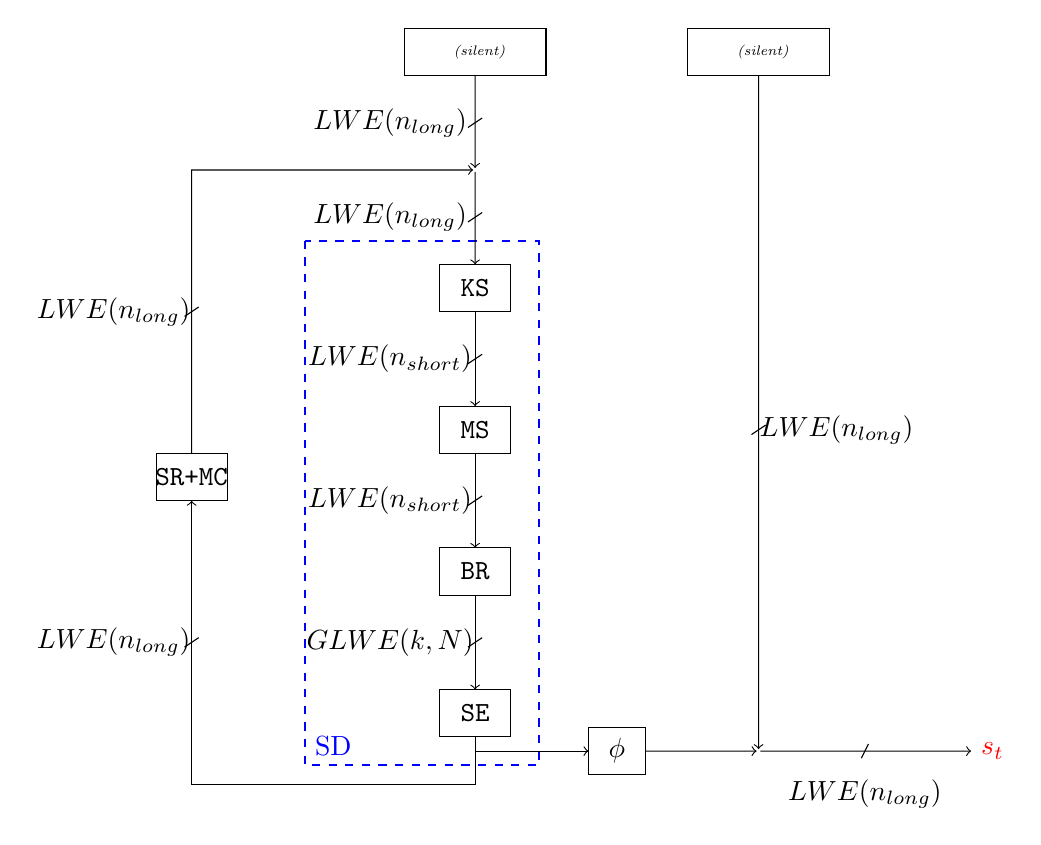
\begin{tikzpicture}[xscale=0.9,yscale=0.6]
 
    %LSFRs
    \draw[] (0, 0) rectangle (2, 1) node[pos=0.5]{$\pseudoKS$ {\tiny \emph{(silent)}}} ;
    \draw[] (4, 0) rectangle (6, 1) node[pos=0.5]{$\whitening$ {\tiny \emph{(silent)}}} ;
    \draw (1, -2) node[inner sep=0pt](addm){$\boxplus$} ;
    \draw[->] (1, 0) -- (addm);

    % FSM
    \draw[] (0.5, -4) rectangle (1.5, -5) node[pos=0.5,color=black](ks){$\texttt{KS}$} ;
    \draw[] (0.5, -7) rectangle (1.5, -8) node[pos=0.5,color=black](ms){$\texttt{MS}$} ;
    \draw[] (0.5, -10) rectangle (1.5, -11) node[pos=0.5,color=black](br){$\texttt{BR}$} ;
    \draw[] (0.5, -13) rectangle (1.5, -14) node[pos=0.5,color=black](se){$\texttt{SE}$} ;
    \draw[] (-3.5, -8) rectangle (-2.5, -9) node[pos=0.5,color=black](srmc){$\texttt{SR+MC}$} ;

    % Draw dashed blue box for SB
    \draw[dashed, blue, thick] (-1.4, -3.5) rectangle (1.9, -14.6);
    \node[blue] at (-1, -14.2) {SD}; % Label for the box

    % FSM connections
    \draw[->] (addm) -- (1, -4);
    \draw[->] (1, -5) -- (1, -7);
    \draw[->] (1, -8) -- (1, -10);
    \draw[->] (1, -11) -- (1, -13);
    \draw[->] (1,-14) -- (1, -15) -- (-3, -15) -- (-3, -9);
    \draw[->] (-3, -8) -- (-3, -2) -- (addm);

    % Extraction
    \draw (5, -14.3) node[inner sep=0pt](addr){$\boxplus$} ;
    \draw[] (2.6, -13.8) rectangle (3.4, -14.8) node[pos=0.5,color=black]{$\phi$} ;

    \draw[->] (1, -14.3) -- (2.6, -14.3);
    \draw[->] (3.4, -14.3) -- (addr);
    \draw[->] (5, 0) -- (addr);
    \draw[->] (addr) -- (8, -14.3);
    \draw[color=red] (8.3, -14.3) node(s){$s_t$} ;



    % Wire type
    \draw (0.9, -1.1) -- (1.1, -0.9) ;
    \draw (-0.2, -1) node{$LWE(n_{\text{long}})$} ;
    \draw (0.9, -3.1) -- (1.1, -2.9) ;
    \draw (-0.2, -3) node{$LWE(n_{\text{long}})$} ;
    \draw (0.9, -6.1) -- (1.1, -5.9) ;
    \draw (-0.2, -6) node{$LWE(n_{\text{short}})$} ;
    \draw (0.9, -9.1) -- (1.1, -8.9) ;
    \draw (-0.2, -9) node{$LWE(n_{\text{short}})$} ;
    \draw (0.9, -12.1) -- (1.1, -11.9) ;
    \draw (-0.2, -12) node{$GLWE(k, N)$} ;
    \draw (-3.1, -12.1) -- (-2.9, -11.9) ;
    \draw (-4.1, -12) node{$LWE(n_{\text{long}})$} ;
    \draw (-3.1, -5.1) -- (-2.9, -4.9) ;
    \draw (-4.1, -5) node{$LWE(n_{\text{long}})$} ;
    \draw (4.9, -7.6) -- (5.1, -7.4) ;
    \draw (6.1, -7.5) node{$LWE(n_{\text{long}})$} ;
    \draw (6.45, -14.45) -- (6.55, -14.15) ;
    \draw (6.5, -15.2) node{$LWE(n_{\text{long}})$} ;

    \end{tikzpicture}
  \vspace{1em}
  \hfill~
  \caption{\label{fig:structure_fhe} Types and shapes of ciphertexts in homomorphic \coolName. The $\subWords$ is broken down into its elementary components}
\end{figure}


% Leo: ce qui suit est pour qu'emacs compile bien l'article, pas touche !
%%% Local Variables:
%%% mode: latex
%%% ispell-local-dictionary: "english"
%%% TeX-master: "../main"
%%% End:




	
}
\fi





\ifeprint{


}
\else{
	\subsection{Concrete Parameters}
	\label{sec:concrete_parameters}
	
	Table \ref{tab:transistor_parameters} shows the parameters used for our experiments, all ensuring 128 bits of security. The obtained security levels $\lambda_{\text{short}}$ et $\lambda_{\text{long}}$ have been estimated using the \texttt{lattice estimator}~\cite{lattice-estimator}.
	
	\begin{table}
		\centering
		\caption{\gls{TFHE} Parameters used in our experimentations}.
			\label{tab:parameters}
		\renewcommand{\arraystretch}{1.3}  % Adjust row spacing
		\scalebox{1}{
			\begin{tabular}{|c||*{12}{>{\centering\arraybackslash}p{0.8cm}|}}
				\hline
				$p_{\text{err}}$ & $q$ & $n_{\text{short}}$ & $k$ & $N$ & $\sigma_{\text{short}}$ & $\sigma_{\text{long}}$ & $B_{BR}$ & $\ell_{\text{BR}}$ & $B_{KS}$ & $\ell_{\text{KS}}$ & $\lambda_{\text{short}}$ & $\lambda_{\text{long}}$\\
				\hline
				$2^{-40}$ & $2^{64}$ & 788 & 2 & 1024 & $2^{47}$ & $2^{14}$ & $2^{23}$ & 1 & $2^4$ & 3 & 131.8 & 128.9\\
				\hline
				$2^{-128}$ & $2^{64}$ & 774 & 1 & 2048 & $2^{47}$ & $2^{14}$ & $2^{23}$ & 1 & $2^3$ & 5 & 131.8 & 128.9\\
				\hline
		\end{tabular}}
		
	\end{table}
}
\fi

\ifeprint{
	
}
\else{
	\subsection{Detailed Homomorphic Implementations}
	\label{sec:detailed_implementation}
	
	In the following, we provide a more detailed way of how we implemented the homomorphic version of \coolName.
	
	\paragraph{Homomorphic evaluation of LSFRs.}
	The \coolName design involves two LSFRs operating on elements of $\field{17}$. The standard way to implement an LSFR is to evaluate the linear feedback function on the state at each clock cycle, thus producing a new element that enters the state, while the state is shifted to output an element. 
	%generate the new element at each clock cycle, and then to mutate the state by shifting the elements of the state and compute the linear combination of the state with the coefficients of retroaction to produce a new one.
	We suggest the \emph{silent LFSR} approach for the homomorphic evaluation of LFSRs. In this approach, the encrypted LFSR state is immutable to avoid any noise growth in the underlying ciphertexts (hence keeping the LFSR ``silent''). We use the fact that every output element of the LFSR can be expressed as a linear combination of the initial state. So, at each clock cycle, we compute \emph{in the clear} the coefficients of this linear combination and homomorphically evaluate it on the immutable encrypted state. This process is depicted in Algorithm~\ref{alg:lsfr}.
	
	\begin{algorithm}[t!]
    \caption{\texttt{LFSR.clock} - Produce a pseudo random element of the state. \label{alg:lsfr}}
    
    \KwIn{
        $\left\{
        \begin{aligned}
            &\ell: \text{ Size of the state of the LFSR.} \\
            &(u_1, \dots, u_\ell): \text{ Encrypted initial state of the LFSR.} \\
            &(\lambda_1^{(0)}, \dots, \lambda_\ell^{(0)}): \text{ Coefficients of retroaction in the definition of the LFSR.} \\
            &(\lambda_1^{(i)}, \dots, \lambda_\ell^{(i)}): \text{ Previous coefficients used in the linear combination.}
        \end{aligned}
        \right.$
    }

    \KwResult{
        $\left\{
        \begin{aligned}
            &o^{(i)}: \text{ Encryption of the $i$-th pseudorandom element of $\F_{17}$.} \\
            &(\lambda_1^{(i+1)}, \dots, \lambda_\ell^{(i+1)}): \text{ Updated coefficients of the linear combination.}
        \end{aligned}
        \right.$
    }

    % Add vertical space and horizontal line
    \vspace{0.5em} % adjust the space as needed
    \hrule
    \vspace{0.5em} % adjust the space as needed

    $o^{(i)} \gets 0$

    \Comment{Evaluation of the linear combination}
    \For{$k \in \{1, \dots, \ell\}$}{
        $o^{(i)} \gets \texttt{SumTFHE}(o^{(i)}, \texttt{ClearMultTFHE}(u_k, \lambda_k^{(i)}))$
    }
    \Comment{Update of the next coefficients}
    \For{$k \in \{2, \dots, \ell\}$}{
        $\lambda_k^{(i+1)} \gets \lambda_{k-1}^{(i)} + \lambda_\ell^{(i)} \cdot \lambda_k^{(0)}$
    }
    $\lambda_1^{(i+1)} \gets \lambda_\ell^{(i)} \cdot \lambda_1^{(0)}$
    
    \Return{$o^{(i)}$}
    
\end{algorithm}


	
	%Calling Algorithm \ref{alg:lsfr} (\texttt{LFSR.clock}) several times yields an encrypted stream of pseudorandom elements $(o^{(0)}, o^{(1)}, \dots)$.
	
	\paragraph{Homomorphic evaluation of} \coolName. The complete homomorphic evaluation of a round of one clock cycle of \coolName is depicted in Algorithm~\ref{alg:transistor}, using $\pseudoKS.\texttt{clock}$ and $\whitening.\texttt{clock}$ as subroutines (i.e., Algorithm~\ref{alg:lsfr} evaluated on the key schedule and whitening LFSRs). The most computation intensive part of the algorithm is by far the evaluation of the \gls{PBS} in $\subWords$ which can be fully parallelized to reduce the latency.
	
	\begin{algorithm}[t!]
    \caption{\texttt{Transistor.clock} - Produce $r$ encypted elements of the key stream}
    \label{alg:transistor}
    
 
    \KwIn{
        $\left\{
        \begin{aligned}
        	&\mathcal K: \text{the LFSR used for the pseudo-keyschedule and its state (cf Algorithm \ref{alg:lsfr}).}\\
            &\mathcal W: \text{the LFSR used for the whitening.}\\	
            &X = \left ( \begin{array}{ccc}
            x_{1,1} & \dots & x_{1,\sqrt{m}}\\
            \dots & \dots & \dots\\
            x_{\sqrt{m},1} & \dots & x_{\sqrt{m},\sqrt{m}}\\
            \end{array} \right ): \text{ Encrypted state of the FSM} \\
        \end{aligned}
        \right.$
    }

    \KwResult{
        $\left\{
        \begin{aligned}
            &Y = (y_1, \dots, y_r): \text{ Encryption of $r$ elements of the  key stream } \\
        \end{aligned}
        \right.$
    }

    % Add vertical space and horizontal line
    \vspace{0.5em} % adjust the space as needed
    \hrule
    \vspace{0.5em} % adjust the space as needed

    \Comment{Compute the pseudo-key schedule and adds it to the FSM}
    \For{$i \in [1, \sqrt m]$}{
        \For{$j \in [1, \sqrt m]$}{
            $k_{i,j} \gets \pseudoKS.\texttt{clock}()$\\
            $x_{i,j} \gets \texttt{SumTFHE}(x_{ij}, k_{i,j})$\\
        }
    }
    \Comment{Compute $\subWords$ with a layer of PBS}
    \For{$i \in [1, \sqrt m]$}{
        \For{$j \in [1, \sqrt m]$}{        
            $x_{i,j} \gets \texttt{PBS\_TFHE}(x_{i,j}, S)$\\
        }
    }
    \Comment{Extract the output bits and whiten them}
    $(y_1, \dots, y_r) \gets \phi(X)$\\
    \For{$i \in [1, r]$}{
        $w_i \gets \whitening.\texttt{clock}()$\\
        $y_i \gets \texttt{SumTFHE}(y_i, w_i)$\\
    }
    \Comment{Compute $\shiftRows$, (same as in clear)}
    $X \gets \shiftR(X)$

    \Comment{Compute MixColumns}
    \For{$i \in [1, \sqrt m]$}{
        \For{$j \in [1, \sqrt m]$}{
            $z_{i, j} \gets 0$\\
            \For{$k \in [1, \sqrt m]$}{
                $z_{i, j} \gets \texttt{SumTFHE}(z_{i, j}, \texttt{ClearMultTFHE}(x_{k, j}, MC_{i, k}))$\\
            }
        }
    }

    \Return{$Y$}

\end{algorithm}


	}
\fi

\ifeprint{

}
\else{
	\subsection{Size of the server key}
	\label{sec:server_key_sizes}
	We  provide the sizes for the server keys in Table \ref{tab:server_key_size}, namely the \emph{key-switching key} (KSK) and the \emph{bootstrapping key} (BSK) while using the ciphertext compression technique described in Section~\ref{sec:key_wrapping}. Those keys are only generated and communicated to the server once (during some user enrolment step).
	
	
	
	\begin{table}
		\centering
		\caption{Size of the server keys for the two considered sets of parameters. 
			%This is agnostic to the volume of message sent. 
			\label{tab:server_key_size}}
		
		\renewcommand{\arraystretch}{1.2}  % Adjust row spacing
		\scalebox{0.9}{
			\begin{tabular}{|c||*{3}{>{\centering\arraybackslash}p{4cm}|}}
				\hline
				& Theoretical sizes & Sizes for $p_{\text{err}} = 2^{-40}$ & Sizes for $p_{\text{err}} = 2^{-128}$ \\
				\hline
				~KSK~ &  $n_{\text{long}}\cdot l_{\text{KS}} \cdot \log_2 q $ & 49 KB & 82 KB  \\
				\hline
				~BSK~ &  $n_{\text{short}} \cdot l_{\text{BS}} \cdot \log_2 q \cdot N \cdot (k+1)$ & 6.5 MB & 12.7 MB  \\
				\hline
		\end{tabular}}
		
	\end{table}
}
\fi


